\documentclass[dp.tex]{subfiles}
\begin{document}


\titleformat{\chapter}[display]
  {\normalfont\huge\bfseries}{\chaptertitlename\ \thechapter}{20pt}{\Huge}
\titlespacing*{\chapter}
{0pt}{0ex}{0ex}
\titlespacing*{\section}
{0pt}{3ex}{1ex}

%První příloha nebude v obsahu
\addtocontents{toc}{\protect\setcounter{tocdepth}{-1}}

\chapter{Analyzované překlady}
\label{appendix:preklady}
%teď musíme do obsahu dostat odkaz na Přílohy
\addtocontents{toc}{\protect\setcounter{tocdepth}{1}}
\addcontentsline{toc}{chapter}{Přílohy}
%Ale zas zakázat další přílohy v obsahu
\addtocontents{toc}{\protect\setcounter{tocdepth}{-1}}

V této příloze je uveden originální text Havrana Edgara Allana Poea a seznam analyzovaných českých překladů. U každého překladu je uvedena stránka, na které je možné daný překlad najít v \cite{Poe1990}, a text čtrnácté strofy, který byl použit v kapitole \ref{chap:denotation-analysis}. Kompletní znění básní je k dispozici na CD přiloženém k této práci.

\section*{E. A. Poe}

\citetitle{Poe1990}, strana~61.
\\\textbf{Text čtrnácté strofy}
\begin{verse}
Then, methought, the air grew denser, perfumed from an unseen censer\\
Swung by seraphim whose foot-falls tinkled on the tufted floor.\\
“Wretch,” I cried, “thy God hath lent thee — by these angels he hath sent thee\\
Respite — respite and nepenthe, from thy memories of Lenore;\\
Quaff, oh quaff this kind nepenthe and forget this lost Lenore!”\\
\hspace*{0.8cm}Quoth the Raven “Nevermore.”
\end{verse}

\section*{V. K. Šembera}
\citetitle{Poe1990}, strana~85.
\\\textbf{Text čtrnácté strofy}
\begin{verse}
\textit{Její} hlas to byl! — A hle, tu vzduch pln vůně jako z květů\\
 pojednou, snad z jiných světů!? Kouzelně to vonný vzduch!\\
 „Blázne,“ dím a slze roní z očí se mi, „touha po ní\\
 by tě více nemořila, zapomenutí ti bůh\\
 sesílá; máš zapomenout, tím tě obdařuje bůh!“\\
\hspace*{0.8cm}Havran nato: „Nikdy víc.“
\end{verse}

\section*{J. Vrchlický (1890)}
\citetitle{Poe1990}, strana~89.
\\\textbf{Text čtrnácté strofy}
\begin{verse}
 Ve vzduchu se vůně chvěla,\\
 jak by z kaditelnic spěla\\
 Serafů, jichž kroků echo\\
 jizbou znělo zmírajíc.\\
 „Bídný!“ křiknu, „v tvoji těchu\\
 anděly Bůh seslal v spěchu,\\
 by tvá duše v moři vzdechů\\
 nepenthes to lokajíc\\
 na Lenoru zapomněla\\
 sladký mok ten lokajíc.“\\
\hspace*{0.8cm}Na to Havran: „Nikdy víc!“
\end{verse}

\section*{J. Vrchlický (1881)}
\citetitle{Poe1990}, strana~172.
\\\textbf{Text čtrnácté strofy}
\begin{verse}
 Ve vzduchu se vůně chvěla, jak by z kaditelnic spěla\\
 andělů, jichž kroků echo znělo chodbou zmírajíc.\\
 „Věru,“ křiknu, „V tvoji těchu anděly bůh seslal v spěchu,\\
 by tvá duše v moři vzdechů nehynula zoufajíc,\\
 Leonoru zapomněla v moři vzdechů zoufajíc!“ —\\
\hspace*{0.8cm}Na to havran: „Nikdy víc!“
\end{verse}

\section*{A. E. Mužík}
\citetitle{Poe1990}, strana~95.
\\\textbf{Text čtrnácté strofy}
\begin{verse}
 Náhle vzduch je dusný, sytý\\
 kadidlem a vůní zpitý,\\
 zachvívá se serafíny,\\
 jichž teď kroky půda zní.\\
 „Nešťastníče,“ křiknu, „nebe\\
 navštívilo dnesky tebe,\\
 ještě můžeš spasit sebe,\\
 rozluč jen svou paměť s ní,\\
 pij z poháru zapomnění,\\
 rozluč svoji paměť s ní —“\\
 Kváče havran: „Nadarmo!“
\end{verse}

\section*{K. Dostál-Lutinov}
\citetitle{Poe1990}, strana~101.
\\\textbf{Text čtrnácté strofy}
\begin{verse}
 Pak jsem cítil dým a vůně. Rostly v kaditelen lůně,\\
 jimiž mával neviděný Serafínů letmých sbor.\\
 „Ubožáku,“ volám křiče, „anděly Bůh seslal z výše,\\
 dal ti pít z Nepenthy číše zapomnění na Lenor!\\
 Vypij číš tu milosrdnou zapomnění na Lenor!“\\
\hspace*{0.8cm}Havran však: „Ne! Nevermore!“
\end{verse}

\section*{V. Nezval}
\citetitle{Poe1990}, strana~108.
\\\textbf{Text čtrnácté strofy}
\begin{verse}
Zdálo se, že u stínidla houstne světlo od kadidla,\\
že se bezpochyby anděl v zvoncích z nebe propadne.\\
„Chudáku, tvůj Bůh ti v zpěvu posílá sem úlevu\\
balzám tvou starou něhu, po němž navždy vychladne\\
po němž láska k Lenoře v tvé mysli navždy zapadne“ –\\
\hspace*{0.8cm}Však havran děl: „Už víckrát ne.“
\end{verse}

\section*{O. F. Babler}
\citetitle{Poe1990}, strana~112.
\begin{samepage}
\\\textbf{Text čtrnácté strofy}
\begin{verse}
Vzduch zdál se mi s vůní stmelen, jak by stoupal z kadidelen\\
andělů, jichž krok zněl jizbou – ale jakby odjinud.\\
„Ubožáku bědný,“ děl jsem, „Bůh tvůj tobě poslat chtěl sem\\
po anděli, který spěl sem, balzám, jaký ztiší rmut.\\
Pij ten nápoj zapomnění: po Lenoře ztiš svůj rmut!“\\
Havran krákl: „Marný blud!“
\end{verse}
\end{samepage}

\section*{J. Taufer}
\citetitle{Poe1990}, strana~119
\\\textbf{Text čtrnácté strofy}
\begin{verse}
Vzduch voněl – zdálo se mi – dým nad kaditelnicemi\\
v rukou serafů, jichž kroky zvonily tu dál, tu blíž\ldots\\
„Ubohý!“ já vzkřikl, „Měla serafů ta říše celá\\
zaplašit žal z tvého čela jako zapomnění číš –!\\
Pij, zapomeň na Lenoru, pij -- a zapomeneš spíš\ldots!“\\
\hspace*{0.8cm}Praví havran: „Nikdy již!“
\end{verse}

\section*{E. Stoklas}
\citetitle{Poe1990}, strana~125
\begin{samepage}
\\\textbf{Text čtrnácté strofy}
\begin{verse}
Tajemně tu vzduch se zhustil, kadidla proud vonný vústil,\\
vhoupán serafy, jichž kroky, zvučící jen, nezřel zrak.\\
„Bídný,“ vzkřik jsem, „boží sláva nad tebou se smilovává --\\
anděl klid a mír ti dává -- zapomnění Lory tak!\\
Pij, ó pij to zapomnění, zhosť se mrtvé Lory tak!“\\
\hspace*{0.8cm}Havran řekl: „Nikterak.“
\end{verse}
\end{samepage}

\section*{D. Wagnerová}
\citetitle{Poe1990}, strana~130
\\\textbf{Text čtrnácté strofy}
\begin{verse}
Vtom jak by mi vůně vály,\\
z kaditelnic vystoupaly\\
rozhoupaných serafíny --\\
zlatým zvukem vzduch se třás.\\
„Viz,“ já děl si, „můj ty světe\\,
Bůh tvůj vysvobodit chce tě,\\
posílá ti nápoj z Léthé,\\
už se nepamětí spas!\\
Před Jarmilou rvoucí ve zmar\\
nápojem se z Léthé spas!“\\
Krákne Havran: „Vrátit čas?“
\end{verse}

\section*{R. Havel}
\citetitle{Poe1990}, strana~137
\\\textbf{Text čtrnácté strofy}
\begin{verse}
Vzduch tak zhoustl, zdálo se mi, jemný parfém padal k zemi,\\
andělé jen kroky svými mohli jej tak rozehrát.\\
„Bídný,“ volám, „Bůh tě chrání, křídel andělských ti vání\\
nese nápoj umírání, abys nemoh vzpomínat!\\
Pij jen, pij jen, abys nemoh Leonóru vzpomínat!“\\
\hspace*{0.8cm}Havran řek: „Ni jedenkrát.“
\end{verse}

\begin{samepage}
\section*{J. B. Čapek}
\citetitle{Poe1990}, strana~141
\\\textbf{Text čtrnácté strofy}
\begin{verse}
Vzduch teď houstl, zdálo se mi, zachvíval se pod vůněmi\\
čeřen andělem -- ach, tys to prozradila, ozvěno!\\
Vzkřikl jsem: „Bůh mou bídu mění, seslal nápoj zapomnění,\\
by mně zhaslo v okamžení tvoje jméno, Eleno,\\
pít, pít nápoj konejšivý, zapomenout, Eleno!“\\
Havran: „Stokrát ztraceno.“
\end{verse}
\end{samepage}

\section*{K. Resler (1948)}
\citetitle{Poe1990}, strana~145
\begin{samepage}
\\\textbf{Text čtrnácté strofy}
\begin{verse}
Nenadálý závan vůně vyvstal jako z rajské tůně,\\
ke mroucímu světlu táh se oblak jemných vonných par.\\
„Ubožáku,“ pravím k sobě, „Bůh sem seslal pomoc tobě,\\
abys po tak dlouhé době došel klidu, ztlumil svár,\\
zbyl se touhy po Lenoře, ztlumil svého srdce svár.“\\
\hspace*{0.8cm}Havran krákl: „Marnost -- zmar.“
\end{verse}
\end{samepage}

\section*{K. Resler (1956)}
\citetitle{Poe1990}, strana~193
\begin{samepage}
\\\textbf{Text čtrnácté strofy}
\begin{verse}
Nenadálý závan vůně vyvstal jako z rajské tůně,\\
k mroucímu se světlu táhl oblak jemných vonných par:\\
„Ubožáku! V strasti době Bůh sem seslal pomoc tobě,\\
klid, jen klid už získej sobě, obrať zrak svůj na pohár!\\
Chop, ó chop jej, obrať zrak svůj zapomnění na pohár!“\\
\hspace*{0.8cm}Havran krákl: „Marnost - zmar.“
\end{verse}
\end{samepage}

\begin{samepage}
	\section*{R. Černý}
	\citetitle{Poe1990}, strana~149
	\\\textbf{Text čtrnácté strofy}
	\begin{verse}
	Tu vzduch houstnul, zdálo se mi, kadidlem jak provoněný,\\
	po koberci kráčí Seraf, šíří vůně posvátné\ldots\\
	„Ubožáku, už se utiš, vždyť ti posílá sám Bůh již\\
	po anděli útěchu, jíž žal v tvém srdci vychladne\ldots\\
	Přijmi lék ten, pro Lenoru žal v tvém srdci vychladne.“\\
	\hspace*{0.8cm}Havran děl však: „Nikdá ne!“
	\end{verse}
\end{samepage}

\section*{I. Slavík}
\citetitle{Poe1990}, strana~154
\\\textbf{Text čtrnácté strofy}
\begin{samepage}
\begin{verse}
A když jsem tak oči mhouřil, houstl vzduch, jak dým by kouřil,\\
po kobercích -- andělů slyš lehké kroky obratné.\\
„Ach, to Bůh se slitovává, po těch andělech mi dává\\
poshovění-zapomnění, v něm se láska propadne,\\
pij ten nápoj, Leonora do tmy se v něm propadne!“\\
\hspace*{0.8cm}Pravil havran: „Víckrát ne.“
\end{verse}
\end{samepage}

\section*{S. Kadlec}
\citetitle{Poe1990}, strana~159
\\\textbf{Text čtrnácté strofy}
\begin{verse}
Vzduch v tom zhoustl -- zdálo se mi -- voněl kaditelnicemi\\
Kůrů, jejichž krok zněl zemí, ač se na ni sotva klad.\\
 „Bůh ti,“ vzdychl jsem,  „poslal zhůry népenthesu těmi Kůry,\\
pij ho, rozptyl jím své chmury, nešťastníku, přestaň lkát!\\
Pozapomeň na Lenoru, přestaň věčně nad ní lkát!“\\
\hspace*{0.8cm}Havran krák však: „Nikdykrát!“
\end{verse}

\section*{A. Bejblík}
\citetitle{Poe1990}, strana~163
\\\textbf{Text čtrnácté strofy}
\begin{verse}
Pak vzduch zhoust a vůně, zdá se, z kadidelnic rozlila se\\
rozhoupaných anděly, jejichž krok se půdy sotva tkne.\\
"Ubožáku, bůh ti," povím, "posílá po andělovi\\
omamný mok opiový na tvou lásku k Tereze;\\
pij, ach pij ten nápoj na tvou lichou lásku k Tereze;\\
Havran řekl: Marno vše.
\end{verse}

\chapter{Diagram tříd denotační analýzy}
\label{appendix:class-diagram}

\begin{figure}[H]
	\centering
	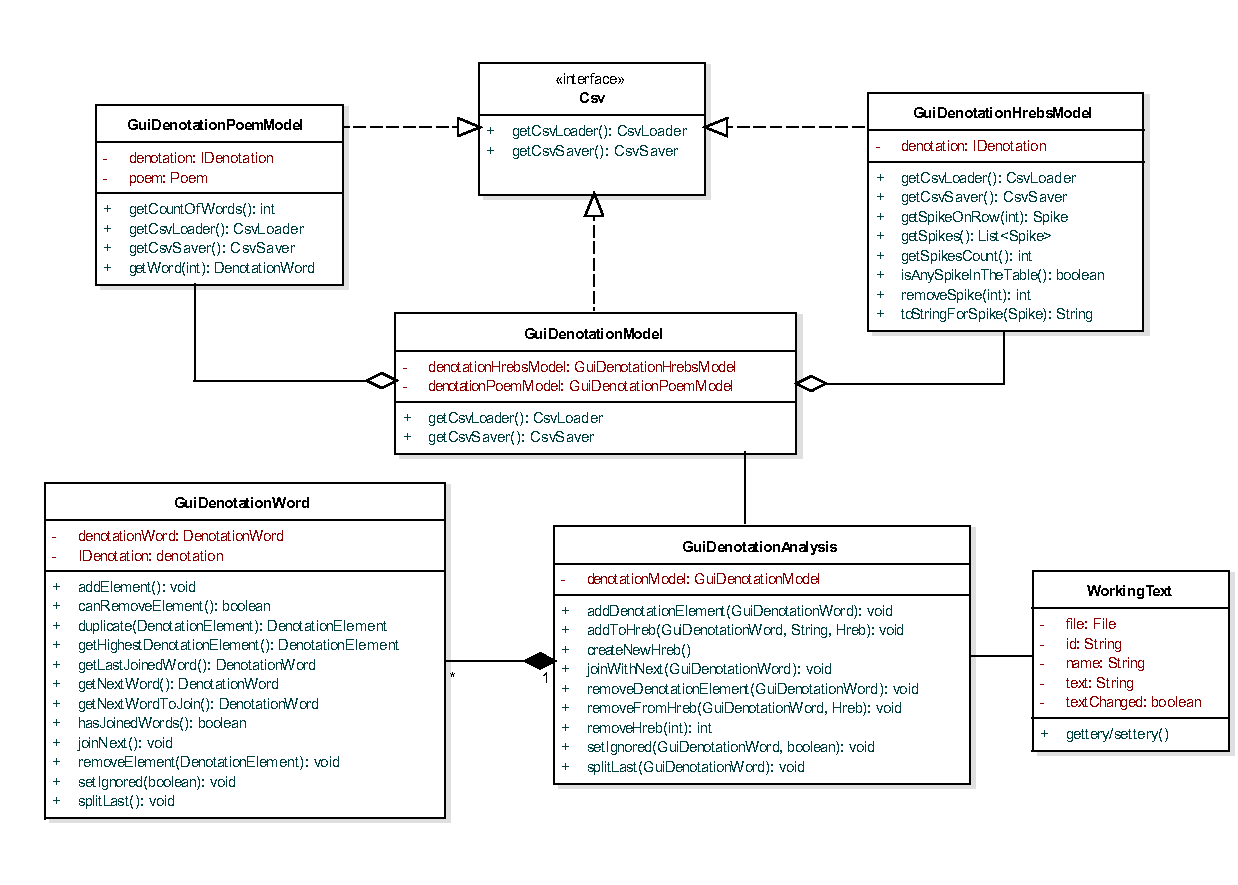
\includegraphics[max width=\textwidth,keepaspectratio=true]{imgs-60-aplikace/gui-denotation-class-diagram}
	\caption[]{Diagram tříd denotační analýzy v modulu grafického uživatelského rozhraní. \textit{Zdroj:~vlastní.}}
	\label{fig:gui-denotation-class-diagram}
\end{figure}


\newpage
\begin{figure}[H]
	\centering
	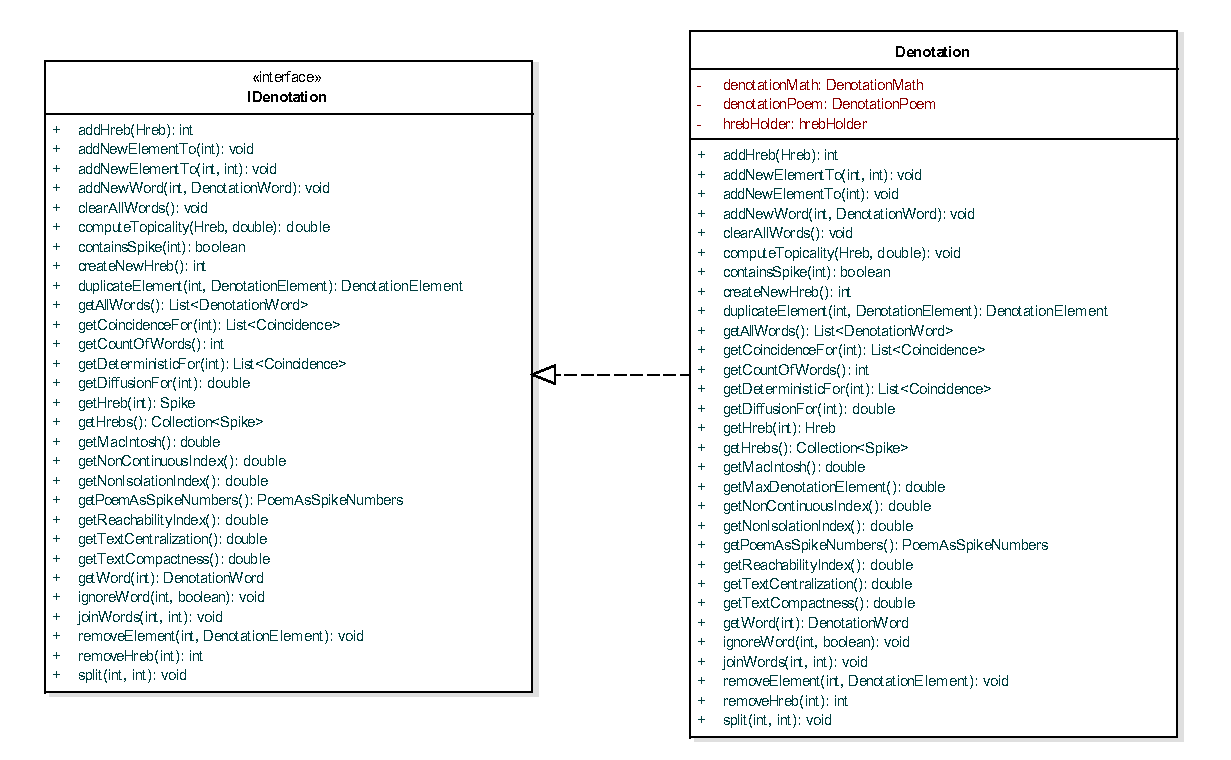
\includegraphics[max width=\textwidth,keepaspectratio=true]{imgs-60-aplikace/compLing-IDenotationInterface-class-diagram}
	\caption[]{Rozhraní \texttt{IDenotation}. \textit{Zdroj:~vlastní.}}
	\label{fig:gui-idenotation-class-diagram}
\end{figure}

\newpage
\begin{figure}[H]
	\centering
	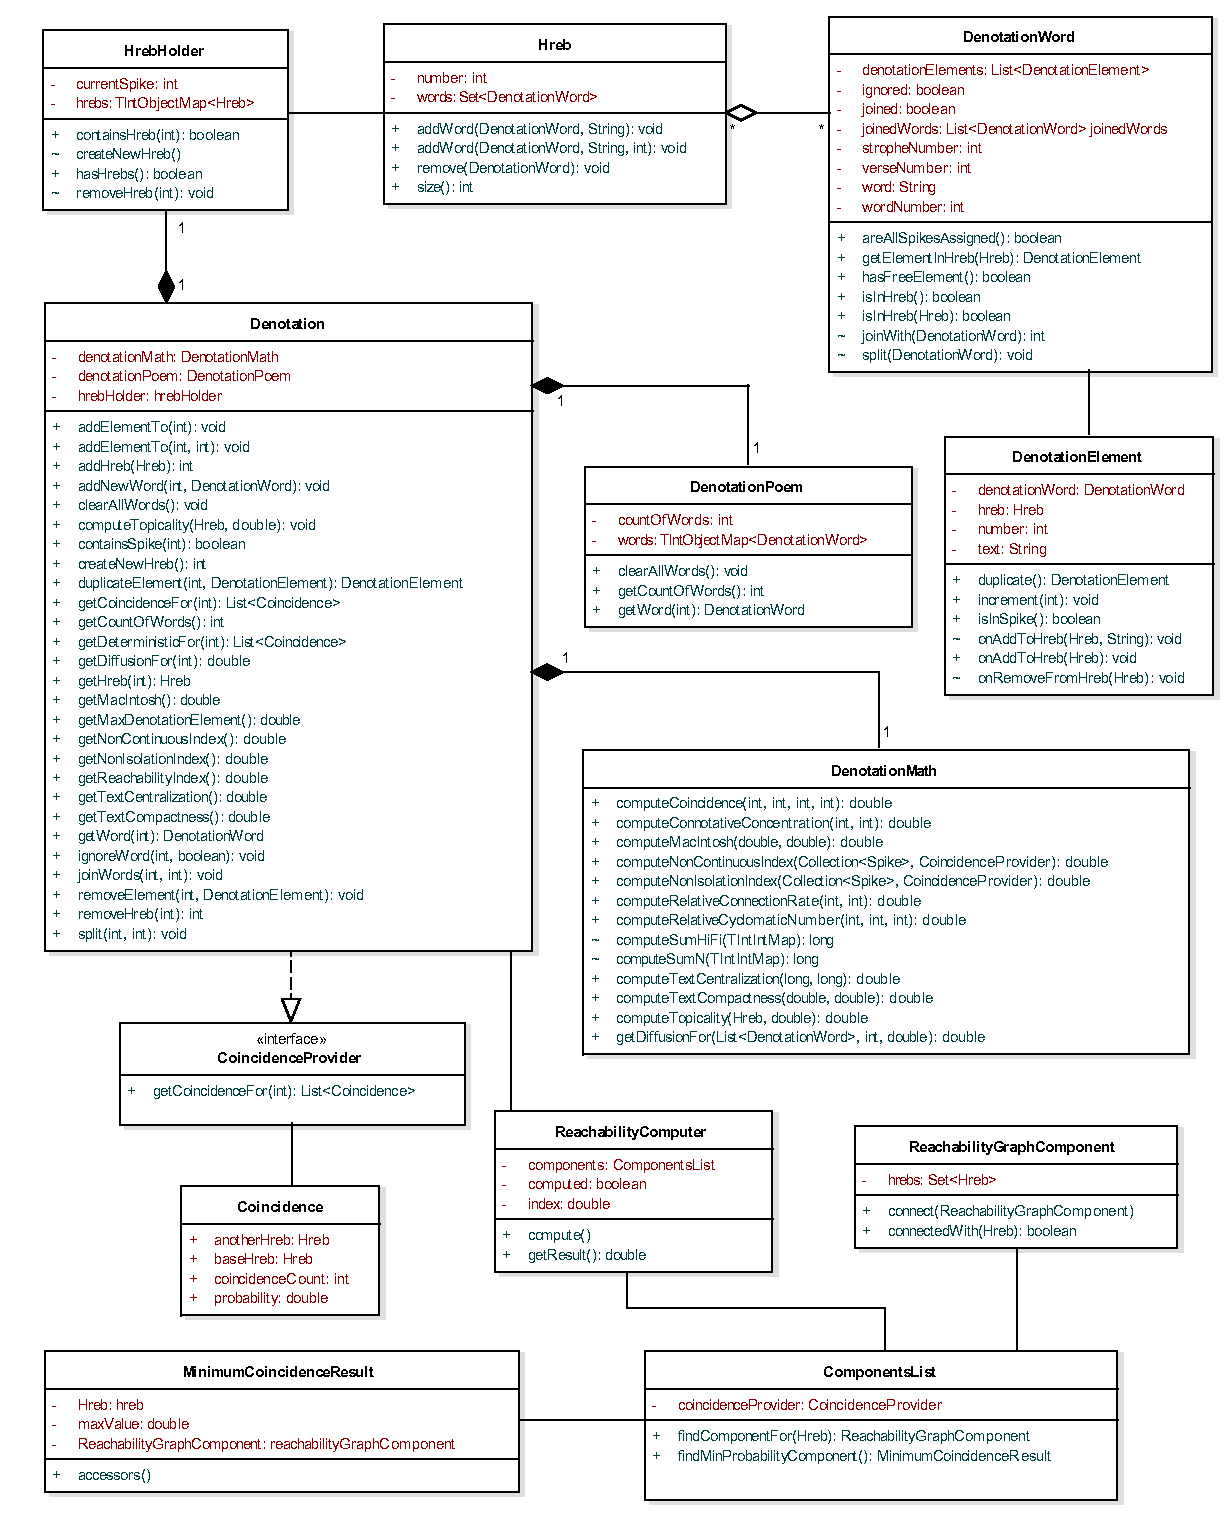
\includegraphics[max width=\textwidth,keepaspectratio=true]{imgs-60-aplikace/compLing-denotation-class-diagram}
	\caption[]{Diagram tříd denotační analýzy v knihovně \texttt{CompLing}. \textit{Zdroj:~vlastní.}}
	\label{fig:compling-denotation-class-diagram}
\end{figure}



\chapter{Ukázka výsledku analýzy asonance}
\label{appendix:asonance}
\begin{figure}[H]
	\centering
	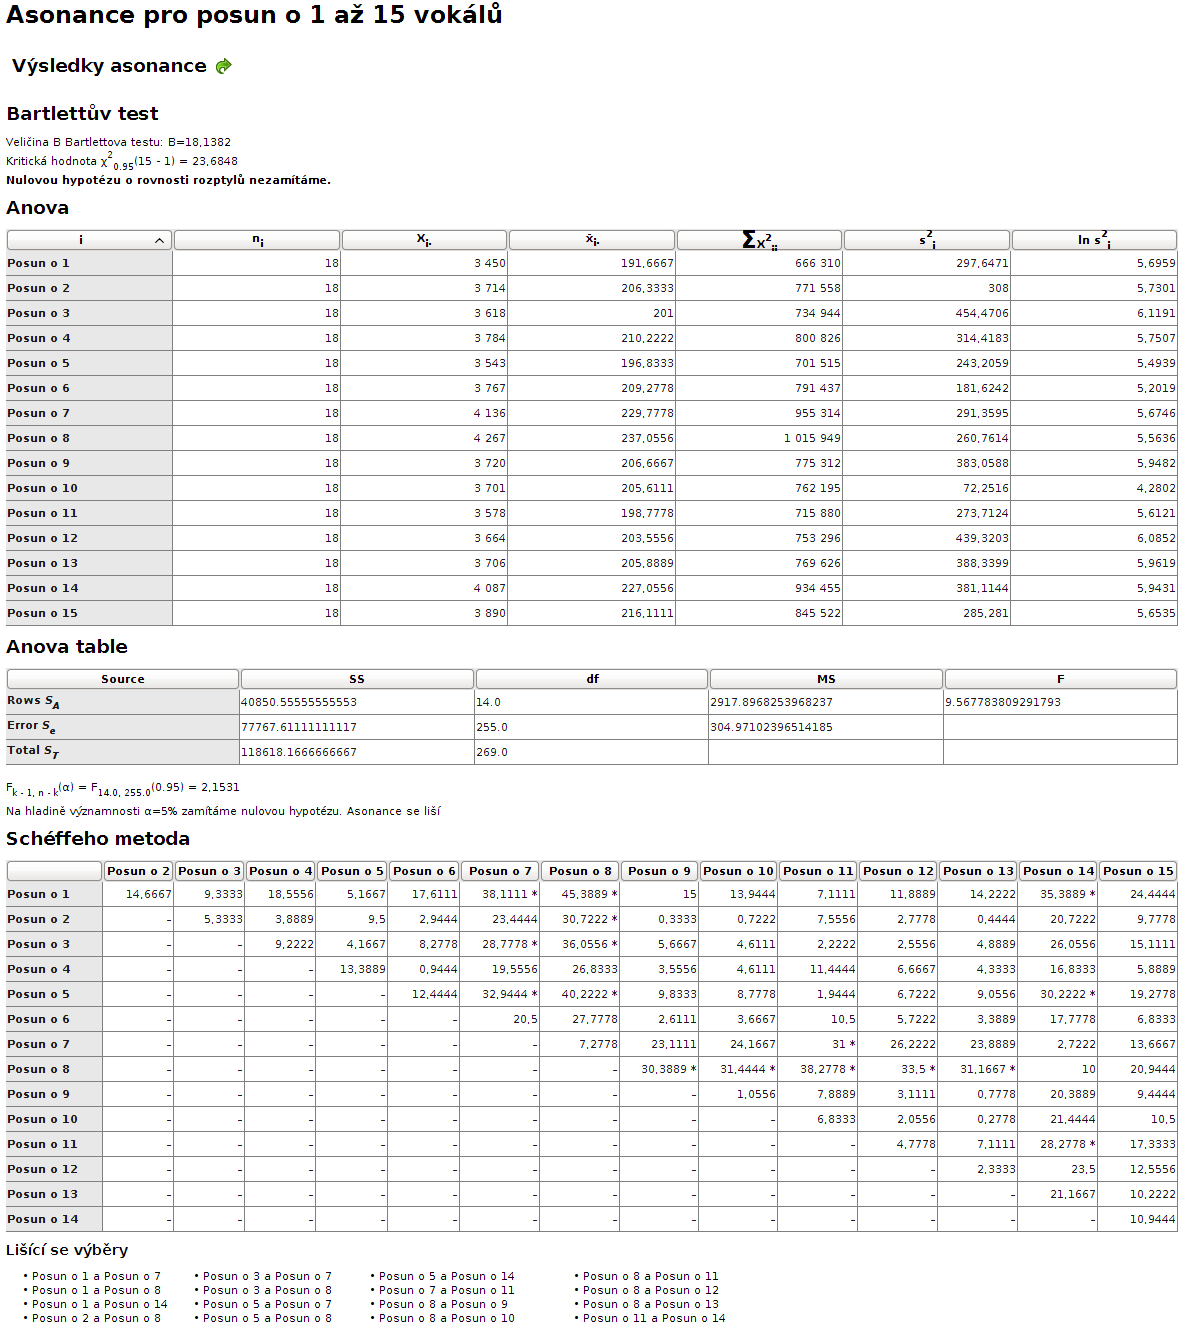
\includegraphics[max width=\textwidth,keepaspectratio=true]{imgs-70-prakticka/assonance}
	\caption[Ukázka výsledku analýzy asonance pro posun o jeden až patnáct vokálů.]{Ukázka výsledku analýzy asonance pro posun o jeden až patnáct vokálů. \textit{Zdroj:~vlastní.}}
	\label{fig:denotation-resler-007}
\end{figure}
\addtocontents{toc}{\protect\setcounter{tocdepth}{3}}
\end{document}
